%
%	introduction.tex
%
%	Proposal Introduction
%
%	John Hughes and Michael Jean
%	University of Manitoba
%

\chapter{Introduction}

\section{Background}

Formula SAE\nomenclature{SAE}{Society of Automotive Engineers} is
an engineering student design competition organized by the Society
of Automotive Engineers dating back to 1978 \cite{fsaehistory}. Students
from the University of Manitoba have participated in the competition
almost every year since 1985. The competition consists of designing
and constructing a small, open-wheeled, formula-style race car.

The Formula SAE vehicle is a performance car built with the primary goal of doing well in the dynamic events at the yearly competitions. These events test the vehicles' abilities in acceleration, braking, and handling.

\subsection{Existing Electrical Systems}

The vehicle as a whole is primarily a mechanical device, but carries several critical electronic control systems.

\begin{figure}[h!]
  \begin{center}
    \subfigure[DTAFast S80]{
      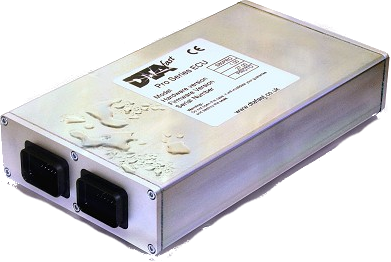
\includegraphics[scale=0.5]{figures/s80.png}
    }
    \subfigure[Race Technology DL1]{
      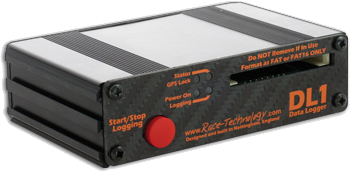
\includegraphics[scale=0.5]{figures/dl1.png}
    }
    \caption{\label{fig:qm/complexfunctions} Existing Electronic Systems.}
  \end{center}
\end{figure}

\subsubsection{ECU}

\nomenclature{ICE}{Internal Combustion Engine}
\nomenclature{ECU}{Engine Control Unit}

The \emph{Internal Combustion Engine} (ICE), a Honda CBR600 F4i, is controlled by an off-the-shelf S80Pro \emph{Engine Control Unit} (ECU) from DTAFast \cite{s60pro}, which controls fuel injection and spark timing signals to the fuel injectors and coils. A feedback path to the ECU from a wide-band oxygen sensor downstream of the combustion chamber allows the controller to sense the amount of residual oxygen in the exhaust, and allows closed-loop control of the combustion process. The ECU also reads several tempurature, pressure, and rotational velocity sensors from the engine.

\subsubsection{DAQ}
\nomenclature{DAQ}{Data Aquisition device, provides and logs high-performance GPS, accelerometer, and ADC input data}
\nomenclature{GPS}{Global Positioning System}

The \emph{Data Aquisition Device} (DAQ) is an off-the-shelf model DL1 from Race Technology \cite{DL1Dsheet}. The DL1 is an expandable data logger with built-in 20-Hz GPS and 3-axis accelerometer. Race Technology provides a software suite that communicates with the DAQ using a documented serial protocol. Every item that the DAQ logs is output in its own channel in real time on the serial line. It is also possible to configure the software to recognize new channels for arbitrary types of data.
Data Aquisition is 

\section{Purpose}

Many of the issues that directly affect the teams' performance at
competition relate to driver training, feedback, and the tuneability
of the car. Most of the mechanical systems on the car must currently
be imprecisely hand-tuned, and are packaged in hard to reach places,
and require body panels or the seat to be removed for access.

Our overall goal is thus to improve the precision, adjustability, and
repeatability of adjustment, of various important mechanical systems
in the car, and to improve the efficiency of testing. We want a shorter
driver feedback-tuning loop in order to eliminate
overshoot and undershoot in tuning, and to avoid other external disturbances.

A second major goal is to improve upon the transmission control systems
of previous years' designs.

% For example, tuning the suspension for a given ride height and road
% surface requires the driver to drive several laps, and then adjust
% damping rates on the dampers by hand with a screw driver, a half-turn
% at a time. This is imprecise, since there is no quantification of
% the actual damping rate that gets dialed in, and is typically unrepeatable
% if conditions change and the team wants to readjust the suspension.
% It's also not feasable to adjust the suspension for each seperate
% drivers preferences.

\section{Methods Used}

We aim to meet our goals by designing and building a decentralized CAN
automotive network with a series of specialized modules that will interface
with each other, as well as with their own actuators and sensors.